\section{General Overview}

\begin{frame}{Parametrized Partial Differential Equations}
    \begin{block}{RB Problem}
        Rectangular parameter space $\mathcal{P} := \{ \mu \in \mathbb{R}^d \; | \; {(\mu_a)}_i \leq \mu_i \leq {(\mu_b)}_i, i = 1, \dots, d \}$

        Find a solution $u \in V$ for
        \begin{equation*}
            a_\mu(u, v) = l_\mu(v) \qquad \forall v \in V
        \end{equation*}
    \end{block}
    \begin{itemize}
        \item $a_\mu$: continuous, coercive, bilinear, \textbf{parameter separable}, and
        \item $l_\mu$: continuous, linear, \textbf{parameter separable}.   
    \end{itemize}
\end{frame}

\begin{frame}{Optimization over Parameter Domain}
    \begin{block}{Parameter Optimization}
        \vspace*{-8pt}
        \[ \min\limits_{\mu} \mathcal{J}(u, \mu) \]
    \end{block}
    \[ \mathcal{J}(u, \mu) := \Theta(\mu) + j_\mu(u) + k_\mu(u, u) \]
    \begin{itemize}
        \item $k_\mu$: continuous, symmetric, bilinear,
        \item $j_\mu$: continuous, linear, and
        \item $\Theta$: arbitrary parameter function.
    \end{itemize}
\end{frame}

\begin{frame}{Adaptive Approach}
    \begin{columns}
        \column{0.5\linewidth}
            \begin{figure}
                \centering
                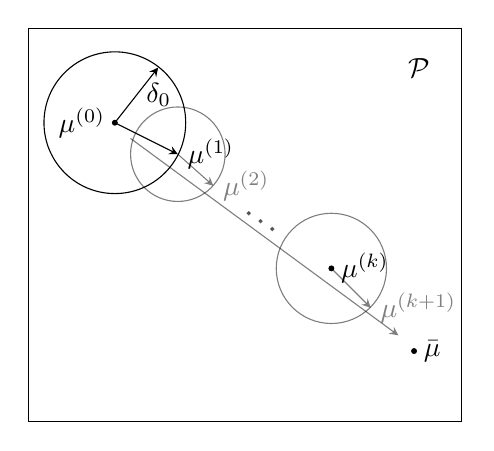
\begin{tikzpicture}[>=stealth]
                    \draw[fill=white] (-2.5,-2) rectangle (3,3);
                    \draw[black](2.2,2.5) node[right] (scrip) {$\mathcal{P}$};
                    \draw[fill=black] (-1.4,1.8) circle [radius=0.03, color=black];
                    \draw[black](-1.4,1.8) node[left] (scrip) {$\mu^{(0)}$};
                    \draw[fill=black] (2.4,-1.1) circle [radius=0.03, color=black];
                    \draw[black](2.4,-1.1) node[right] (scrip) {$\bar{\mu}$};
                    %\draw[->] (-1.2,1.6) -- (1.8,-0.9) node; %[midway,right] {Optimization};
                    \draw[->, opacity=0.5] (-1.2,1.6) -- (2.2,-0.9) node {}; %[midway,right] {Optimization};
                    \draw[->,black] (-1.4,1.8) -- (-0.85,2.5) node [midway,right] {$\delta_0$};
                    \draw[black] (-1.4,1.8) circle [radius=0.9, color=black];
                    \draw[->,black] (-1.4,1.8) -- (-0.6,1.4) node [right] {$\mu^{(1)}$};
                    \draw[black, opacity=0.5] (-0.6,1.4) circle [radius=0.6, color=black];
                    \draw[->,black, opacity=0.5] (-0.6,1.4) -- (-0.15,1) node [right] {$\mu^{(2)}$};
                    %\draw[fill=black, opacity=0.5] (0,0.85) circle [radius=0.03, color=black];
                    %\draw[fill=black, opacity=0.5] (0.15,0.75) circle [radius=0.03, color=black];
                    \draw[fill=black, opacity=0.5] (0.3,0.65) circle [radius=0.02, color=black];
                    \draw[fill=black, opacity=0.5] (0.45,0.55) circle [radius=0.02, color=black];
                    \draw[fill=black, opacity=0.5] (0.6,0.45) circle [radius=0.02, color=black];
                    \draw[fill=black] (1.35,-0.05) circle [radius=0.03, color=black];
                    \draw[black](1.35,-0.05) node[right] (scrip) {$\mu^{(k)}$};
                    \draw[black, opacity=0.5] (1.35,-0.05) circle [radius=0.7, color=black];
                    \draw[->,black, opacity=0.5] (1.35,-0.05) -- (1.85,-0.55) node [right] {$\mu^{(k+1)}$};
                \end{tikzpicture}
                \caption{Local adaptation (TR) on the domain,\\figure courtesy of Tim Keil}
            \end{figure}
        \column{0.5\linewidth}
            \only<2>{
                \begin{algorithm}[H]
                    \While{not converged}{
                        Compute locally optimal solution\;
                        
                        \If{some condition}{
                            Continue to next optimization step\;
                        }
                        \Else{
                            Change some parameter of the problem\;
                            Optimize again\;
                        }
                    }
                \end{algorithm}
            }

            \only<3>{
                \begin{algorithm}[H]
                    \While{not converged}{
                        Compute locally optimal solution\;
                        
                        \If{some condition}{
                            Continue with refinement\;
                        }
                        \ElseIf{some other condition}{
                            Repeat optimization step with smaller domain\;
                        }
                        \ElseIf{some third condition}{
                            Refine and possibly repeat optimization step\;
                        }
                    }
                \end{algorithm}
            }

            \only<4>{
                \begin{block}{Benefits of the Adaptive Approach}
                    We only adapt locally. \\~\\

                    We \textbf{do not} construct a reduced basis for the entire domain $\mathcal{P}$!
                \end{block}
            }
    \end{columns}
\end{frame}